% ML Final Group Project -- Online News Popularity (v19 storyline: what can be called before publication)
% Limit: 8 pages INCLUDING figures and references. The v18 report is kept in report/v18/main.tex.
\documentclass[10pt,a4paper,twocolumn]{article}
\usepackage[margin=1.9cm]{geometry}
\usepackage{graphicx,booktabs,amsmath,hyperref,xcolor,caption}
\usepackage[numbers,sort&compress]{natbib}
\graphicspath{{../results/figures/}}
\captionsetup{font=small}
\setlength{\textfloatsep}{8pt plus 2pt minus 2pt}

\title{What Can Be Called Before Publication?\\
Platform Signals, Headlines and the Limits of Prediction in Online News Popularity}
\author{Group 3 \\ Machine Learning (6012B0809Y), University of Amsterdam}
\date{December 2026}

\begin{document}
\maketitle

\begin{abstract}
An editor who decides which of the day's articles to push needs to know what can be called before publication,
and from what. We study this on the Mashable benchmark, to which we add the real headlines of 39{,}619 of its
39{,}643 articles, recovered from the publisher's sitemap. Under a strictly past-only protocol, a gradient-boosted
model on the benchmark's features ranks the day's articles with a Spearman correlation of 0.40, its top pick
of the day lands in that day's top tenth 36\% of the time (11\% by chance), and it orders two articles from the
same day and section correctly 61\% of the time. This skill sits in the article rather than its context, and
most of it comes from platform history: how earlier articles with the same keywords did. The headline is a different matter, and its story has two halves. From June 2013 on, it adds nothing we can
detect for telling which of two articles will be shared more: supervised text models on the real headlines and a
zero-shot decision model (JEV, via its API and as an open-weights 9B model) are at chance (49--51\%), in six
different tests. Before that, it was the best single signal: in March--May 2013 a past-only headline model orders
same-day same-section pairs correctly 60\% of the time, better than all 58 features, and the zero-shot judge 59\%;
within days of 7 June 2013 both fall to chance and stay there. The break is in the benchmark itself (the URL keywords
show it too), no feature explains it, and the judge's early signal survives rewording every headline, so it is not
recall. Within one article the headline clearly matters: on randomized headline tests (Upworthy) the same judge is
right 66\% of the time, and 85\% on the quarter of pairs it is most confident about. Most of the variance is not explained by these data:
the model, the day's context and the story together account for about a quarter of the variance of log shares. Choosing the headline is a separate, within-article decision; there an archive of 18{,}200
observational headlines is worth about 1{,}000 randomized tests.
\end{abstract}

% ------------------------------------------------------------------
\section{Introduction}
Every day an editor decides which new articles to promote. Popularity prediction before publication is meant to
support that decision, and the Online News Popularity dataset \citep{fernandes2015} is its standard benchmark:
39{,}644 Mashable articles with 58 features and their share counts. Work on it mostly compares classifiers;
tree ensembles reach a ROC-AUC of about 0.73--0.74. That number does not say what an editor can call. Shares
depend on platform signals (the section, the day, how earlier articles on the same keywords did), on the
article, on its headline, and on things no dataset records, from promotion to social influence and chance
\citep{salganik2006,martin2016,hofman2017}. Which of these can be read before publication, and how much remains
unexplained?

Two things have kept this question open on the benchmark. It has no text, so the headline, the one part of an
article that editors change most and that recent language models judge with ease, could not be tested; and
its usual random cross-validation lets a model learn from the future. We fix both: we recover the real headline of
99.94\% of the articles from Mashable's public sitemap, and we score every model strictly on articles published
after its training data, with the editor's decisions as metrics (rank the day's lineup, pick the day's top
article, choose between two articles of one section and day).

\paragraph{Research questions.}
\begin{enumerate}\setlength\itemsep{0pt}
  \item[RQ1] How much of an article's popularity can be called before publication, measured on the decisions an
             editor makes?
  \item[RQ2] Where does that skill come from: the context, the story, the article; platform history or content?
  \item[RQ3] What does the headline add? Can supervised text models or a zero-shot decision model call
             popularity from it, across articles and within one article?
  \item[RQ4] For the within-article choice of a headline, how much is an archive of past headlines worth compared
             with randomized tests?
\end{enumerate}
\noindent Contributions: (i) a headline layer for the Mashable benchmark (40{,}161 sitemap entries, 99.94\% matched,
100 of 100 audited matches correct), released with the code; (ii) a past-only, decision-level account of
what can be called and from which signals, extending the content-versus-context comparison of
\citet{hessel2017}; (iii) a structural break in the benchmark, dated to 7 June 2013, before which headline text is the
best single predictor and after which it carries none; (iv) an evaluation of a zero-shot decision judge
\citep{zheng2023judge,li2026jev} on same-day matched pairs of real headlines: it tracks that break, is not
explained by recall, and is clearly informative within an article; (v) an exchange rate
between an observational headline archive and randomized experiments (half a page, from our earlier analysis).

% ------------------------------------------------------------------
\section{Related Work}
\paragraph{Popularity prediction.} \citet{fernandes2015} introduced the dataset (random forest, AUC 0.73).
Prediction before publication is hard \citep{bandari2012}; early shares help much more \citep{szabo2010}.
Cascade size is only partly predictable even with rich signals \citep{cheng2014,martin2016}, and social influence
makes success partly unpredictable \citep{salganik2006}; \citet{hofman2017} argue for reporting what is
predictable and from what. \citet{hessel2017} compared content and context for posts in the same community and
hour; our within-day and within-section metrics apply the same idea, and equal group AUC in recommender
evaluation \citep{zhou2018}. Items compete for limited attention \citep{wu2007,weng2012}. Active learning on
streams of networked items \citep{yang2014wsdm,yang2014cikm} motivated our strictly past-only evaluation.
\paragraph{Headlines.} Paired designs hold the item fixed: tweets by one author on one link \citep{tan2014},
resubmissions of one image \citep{lakkaraju2013}. On the Upworthy archive of randomized headline tests
\citep{matias2021}, within-test comparisons identify causal headline effects
\citep{gligoric2023,banerjee2025,robertson2023}, and correlational estimates diverge from them
\citep{banerjee2026}. Headline features predict news popularity on social media only modestly \citep{piotrkowicz2017},
also with neural multi-task models \citep{lamprinidis2018}. Predicting the winning headline of a test is hard:
linguistic features reach about 55\% pairwise
accuracy \citep{gligoric2021}, and language models are only somewhat better \citep{ye2024lola}.
\paragraph{Judges.} LLMs are widely used as zero-shot judges \citep{zheng2023judge}. JEV is a decision-only
model that returns calibrated probabilities over typed options instead of text; \citet{li2026jev} propose to
accept its verdict when it is confident and escalate otherwise, and \citet{rao2026jev} compare it with LLM
rubric judges. We ask whether such a judge can call popularity, a question with ground truth.
\paragraph{Observational versus experimental data.} Observational methods can misestimate effects that
experiments measure \citep{lalonde1986,gordon2019}; the two can be combined by correcting an observational
model with experiments \citep{kallus2018}, by shrinkage \citep{rosenman2023}, or by the methods reviewed in
\citep{colnet2024}; \citet{gentzel2019} argue for evaluating with interventional data.

% ------------------------------------------------------------------
\section{Data}
\label{sec:data}
\paragraph{Mashable.} 39{,}643 articles (one row with an impossible token rate removed) published between
7 January 2013 and 27 December 2014, with 58 features: content (words, links, images, videos, 5 LDA topics, 16
sentiment features, title length and sentiment), placement (6 channels, weekday) and history (keyword and
self-reference statistics), and shares recorded once, in January 2015. Shares are heavy-tailed (median 1{,}400,
maximum 843{,}300); we model $\log(1{+}\text{shares})$ and call an article \emph{popular} if it has at least
1{,}400 shares \citep{fernandes2015}. The history features are computed from \emph{other} articles' shares: the
keyword statistics use only articles from earlier days (\texttt{kw\_max\_max} equals the running maximum of earlier
shares for 99.87\% of articles) but take their shares from the collection date, so their value is likely somewhat
optimistic.

\paragraph{Real headlines.} The dataset gives only the URL, whose slug is a shortened headline. Mashable lists
every article with its full headline in monthly sitemap pages (\texttt{mashable.com/sitemap/YYYY/M}). We fetched the
24 pages for 2013--2014 (one request per second, only listing pages, no article pages), giving 40{,}161
headlines, and matched them to the dataset by slug: 39{,}619 of 39{,}643 articles (99.94\%) match; the 24 others
are left out of all headline analyses. In a random audit of 100 matches, all headlines belonged to their article.
Headlines are longer than slugs (median 9 vs.\ 4 words): the slug \emph{aaron-swartz} is the headline ``Technology's
Greatest Minds Say Goodbye to Aaron Swartz''.

\paragraph{Randomized headline tests.} For the within-article question we use the Upworthy Research Archive
\citep{matias2021}: 22{,}743 A/B tests of its confirmatory split (2013--2015). Packages of one test that share image
and lede form a \emph{cell} in which only the headline was randomized; 27{,}921 pairs of headlines in a cell differ
significantly in click-through (two-proportion $|z|>1.96$). These pairs are the ground truth for ``which headline
of this article does better''.

% ------------------------------------------------------------------
\section{Methods}
\label{sec:method}
\paragraph{Past-only protocol.} For every month from July 2013 on, we fit a model on all articles of earlier
months and score that month; 2013-07 to 2014-12 gives 30{,}446 scored articles (30{,}423 with a headline, used for every comparison). The main model is histogram
gradient boosting \citep{friedman2001,ke2017} (HistGB; learning rate 0.03, 15 leaves, 500 iterations) on the 58
features, trained on log shares; in a chronological benchmark it matches a random forest and beats $L_1$
logistic regression and $k$-NN (AUC 0.737 vs.\ 0.736, 0.717, 0.705).

\paragraph{Decision metrics.} Besides ROC-AUC for popular articles we report what an editor would see:
(a) \emph{day ranking}, the Spearman correlation between score and log shares among the articles of one day,
averaged over days; (b) \emph{top pick}, how often the day's top-scored article is in that day's top 10\% by
shares; (c) \emph{pair accuracy}, the share of all pairs of articles from the same day and section (or the same
day) whose order by score matches their order by shares; and (d) pairwise AUC within a context (week, day,
channel, channel$\times$day, same story), which removes skill that only tells contexts apart. Intervals are
bootstraps over publication days (1{,}000 draws, the same for all models, so differences are paired) or over pairs.

\paragraph{Text models.} On the real headlines we fit, under the same protocol, a ridge regression on TF-IDF word
uni- and bigrams, a ridge regression on 768-dimensional bge-base sentence embeddings \citep{xiao2024bge}, and
HistGB on the 58 features plus 32 principal components of the embeddings (fitted on the training months). For
cold start we score each headline's novelty as one minus its highest TF-IDF cosine to the headlines of the
previous 30 days; we also give HistGB six \emph{crowding} features (how many and how similar earlier headlines were
in the previous 1, 3, 7 and 30 days).

\paragraph{Zero-shot judge.} JEV (TypeSafe, version 1.14.0, via its API) answers a typed \emph{choice} question
with a probability for each option and no generated text \citep{li2026jev}. We ask: ``Which of these two articles
was shared more often on social media?'', with a state line naming the site, the date and (for same-section pairs)
the section, and the two headlines as options. Every pair is asked in both orders and the probabilities averaged,
which removes position bias. We judge 4{,}000 random same-day same-section pairs and 4{,}000 same-day pairs; the
same pairs with only the URL keywords; 2{,}000 pairs with the headline plus six dataset features (section,
weekday, words, images, videos, \texttt{kw\_avg\_avg}); and whole-day lineups (``which of these articles was
shared the most'', all of a day's headlines as options, three random orders). On Upworthy we ask which headline
``got the higher click-through rate'' for 2{,}000 significant within-cell pairs and 4{,}000 random within-cell
pairs. As an open-weights check we run
the released student model JEV-9B (a Qwen3.5-9B with a LoRA adapter and a decision head) in 8-bit on CPU, on
400 Upworthy and 400 Mashable section pairs with the same prompts. To check sensitivity to wording, 1{,}000 pairs of
each kind are asked again with a different state line and question. Following \citet{li2026jev}, the judge's
confidence is its larger option probability, and we report accuracy on its most confident 25\% and 10\%. Upworthy
headlines are public, so a judge might have seen them; as a check we restrict to pairs in which neither headline
won its test. For Mashable we reworded both headlines of 250 pairs from January--May 2013 (same meaning, names and
numbers, different wording; the rewordings were written by an AI assistant, Claude, and are released) and asked
again: verbatim recall cannot survive this.

\paragraph{When the headline carries signal.} The main protocol scores articles from July 2013. To see earlier
months we also start the rolling origin in March 2013 (training on at least January and February) and report pair
accuracy by month. To date a change we train one headline model on January--March 2013, compute its correlation
with log shares among each later day's articles, and fit a single least-squares change point.

\paragraph{Supervised headline ranking on Upworthy.} As a supervised reference we train ridge regressions on the
randomized within-cell contrasts with frozen GloVe \citep{pennington2014} or RoBERTa \citep{liu2019roberta}
headline representations, five-fold cross-validated over articles.

\paragraph{A variance bound for headlines across articles.} Suppose the log-share difference of two articles is
$\Delta = h + e$, with a headline part $h$ of standard deviation $\sigma_h$ and an independent rest $e$, and a
judge's score correlates $\rho$ with $h$. For jointly Gaussian variables the probability that the judge orders the
pair correctly is $\tfrac12 + \arcsin(\rho\,\sigma_h/\sigma_\Delta)/\pi$. We take $\rho$ and $\sigma_h$ from
Upworthy (the judge's correlation with the randomized contrasts, and their standard deviation on the logit scale),
$\sigma_\Delta$ from Mashable, and write $\sigma_h = c\cdot\sigma_h^{\text{Upworthy}}$, with $c$ the unknown ratio of
headline effects on Mashable shares to those on Upworthy clicks.

\paragraph{Archive versus experiments (RQ4).} Summarised from our earlier analysis: on Upworthy, a ridge model on
GloVe and 15 headline features is trained either on an observational \emph{archive} (one headline per test with its
week-demeaned click-through) or on the randomized contrasts of $k$ tests; the archive's \emph{exchange rate} $k^*$ is
the number of tests at which experiments alone match the archive's decision accuracy.

\paragraph{Reproducibility.} Seeds are fixed; every number and figure comes from a script in the code
(\texttt{run\_all.sh}); judge outputs are cached and released, and the API key is not.

% ------------------------------------------------------------------
\section{Results}
\label{sec:results}

\begin{table}[t]
\centering\footnotesize
\caption{RQ1: what can be called before publication. Past-only scores, articles of 2013-07 to 2014-12; 95\%
intervals bootstrap days. Pairs: all pairs from the same day and section (or day) with different shares.}
\label{tab:called}
\setlength{\tabcolsep}{3pt}
\begin{tabular}{@{}lccc@{}}
\toprule
 & HistGB & \texttt{kw\_avg\_avg} & chance \\
\midrule
AUC (popular) & 0.724 {\scriptsize[0.718, 0.731]} & 0.639 & 0.5 \\
Day ranking (Spearman) & 0.400 {\scriptsize[0.388, 0.413]} & 0.273 & 0 \\
Top pick in day's top 10\% & 35.6\% {\scriptsize[31.7, 39.6]} & 28.1\% & 11.2\% \\
Pair accuracy, day \& section & 60.9\% {\scriptsize[60.4, 61.4]} & 57.1\% & 50\% \\
Pair accuracy, day & 64.7\% {\scriptsize[64.3, 65.2]} & 59.9\% & 50\% \\
\bottomrule
\end{tabular}
\end{table}

\begin{figure*}[t]
\centering
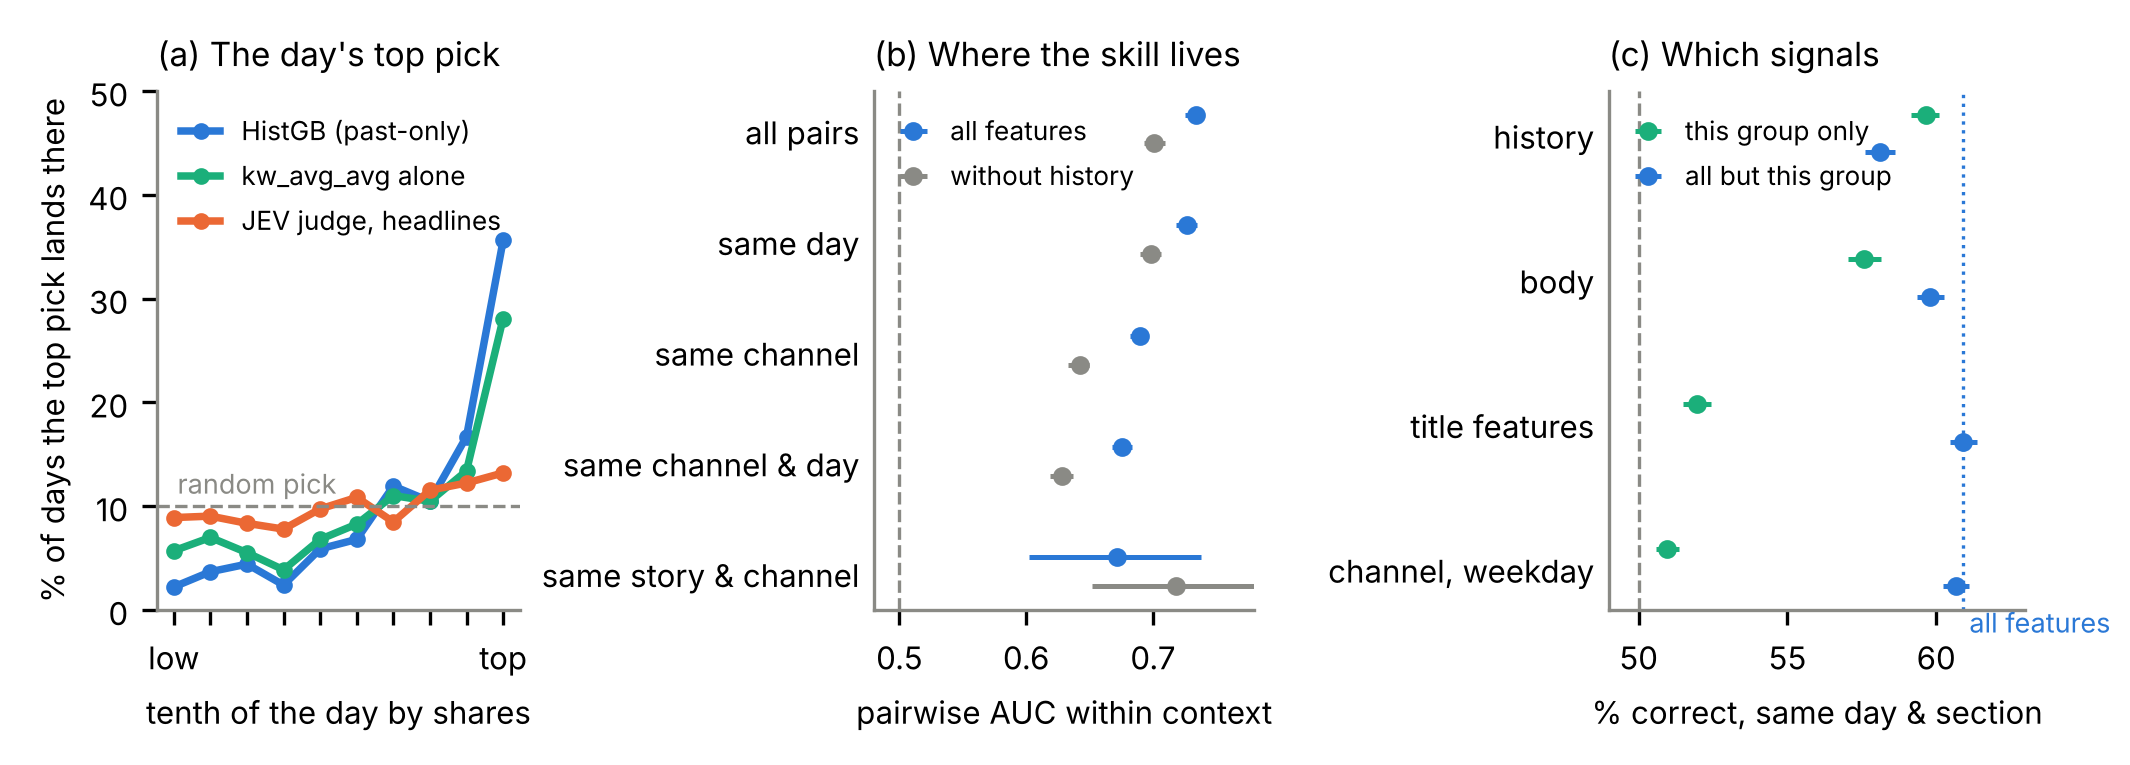
\includegraphics[width=\textwidth]{v19_fig_called.png}
\caption{RQ1--2, past-only scores. (a) Where the article a scorer ranks first each day falls among that day's
articles by shares (tenths; top = at or above the day's 90th percentile); a random pick lands in each tenth about
10\% of the time. (b) Pairwise AUC among articles sharing a context, HistGB classifier with all features and
without the 13 history features (95\% intervals over weeks, or stories). (c) Accuracy on same-day same-section pairs
of HistGB on one feature group alone and on all features but that group (95\% intervals over days).}
\label{fig:called}
\end{figure*}

\subsection{What can be called (RQ1)}
\label{sec:rq1}
Before publication, the day's lineup can be ordered far better than by chance (Table~\ref{tab:called}). Past-only
HistGB reaches an AUC of 0.724 for popular articles, close to the 0.73--0.74 usually reported with random
cross-validation. In the editor's terms: within a day its scores correlate with log shares at 0.40; its top
pick of the day lands in that day's top tenth on 35.6\% of days, three times the 11.2\% of a random pick; and of
two articles from the same day and section it names the more shared one 60.9\% of the time (64.7\% for any two
articles of a day, which can differ in section). A single feature, the average past popularity of the article's
keywords (\texttt{kw\_avg\_avg}), already gets most of the way: 57.1\% on same-day same-section pairs and a top
pick in the top tenth on 28\% of days. For an editor who promotes the past-only model's top pick each day, the pick gets
on average 2.1 [1.9, 2.3] times the shares of a random article of the same day (geometric mean over 545 days)
and beats the day's median article on 79\% of days (its median is 3{,}500 shares; all articles: 1{,}400).

The ceiling is low: most of the variance is not explained by these data. The past-only model explains 16.2\% [15.3, 17.1]
of the variance of log shares; adding fixed effects for channel$\times$day and the story an article belongs to
(same-story articles recovered from near-identical URL slugs, about 71\% precise) raises this to about a quarter
at most. Same-story articles barely share their fate (residual correlation 0.05 [0.02, 0.09]), and articles
compete for the day's attention: on a day with twice as many articles each gets about 18\% fewer shares, an
association that a confounder explaining 4\% of the residual variance would remove.

\subsection{Where it comes from (RQ2)}
\label{sec:rq2}
\paragraph{The article, not its context.} Comparing articles within finer contexts (past-only HistGB
classifier\footnote{A classifier for the popular label, as in our earlier analysis; Table~\ref{tab:called} uses a
regressor on log shares, which ranks articles of a day better but separates the 1{,}400 threshold slightly worse
(AUC 0.724 vs.\ 0.734, same months).}) shows where the skill lives: 0.734 overall, 0.727 within the same day, 0.690 within a channel,
0.675 within channel and day, and 0.672 [0.602, 0.738] for pairs of same-story articles in the same channel.
Knowing which days were good contributes nothing, the channel about 0.045, and holding the story fixed costs at
most about 0.07 more; most of what the model knows is about the article itself.

\paragraph{Mostly platform history.} Refitting past-only HistGB on groups of features (Fig.~\ref{fig:called}c)
shows which signals carry the skill on same-day same-section pairs. The 13 history features alone reach 59.7\%
[59.2, 60.1] of the full model's 60.9\%; the 28 body features alone 57.6\%; the five title features of the
dataset 52.0\%; and channel and weekday, constant within such pairs, 50.9\%. Leaving a group out costs 2.8 points
for history (58.1\%), 1.1 for the body, 0.2 for placement and nothing for the title features. Across all articles the
picture is similar (AUC: history alone 0.682, body alone 0.664, title alone 0.541). History also keeps
the skill alive within contexts: without it, AUC within channel and day falls from 0.675 to 0.628
(Fig.~\ref{fig:called}b). What can be called is therefore mostly how the platform's audience has recently
responded to an article's keywords, some of how the article is built, and almost nothing of its title.

\paragraph{No cold-start penalty, no crowding signal.} Skill does not depend on whether the topic is new:
binned by how similar an article's headline is to any headline of the previous 30 days, AUC is 0.721--0.728 in
all five quintiles (most novel: 0.722). 19\% of articles have a similar headline (cosine $\geq$0.3) in the
previous week, but six ex-ante crowding features change AUC by $-$0.0003 [$-$0.0011, 0.0005] and pair accuracy
by $-$0.0002.

\subsection{What the headline adds (RQ3)}
\label{sec:rq3}
\begin{figure*}[t]
\centering
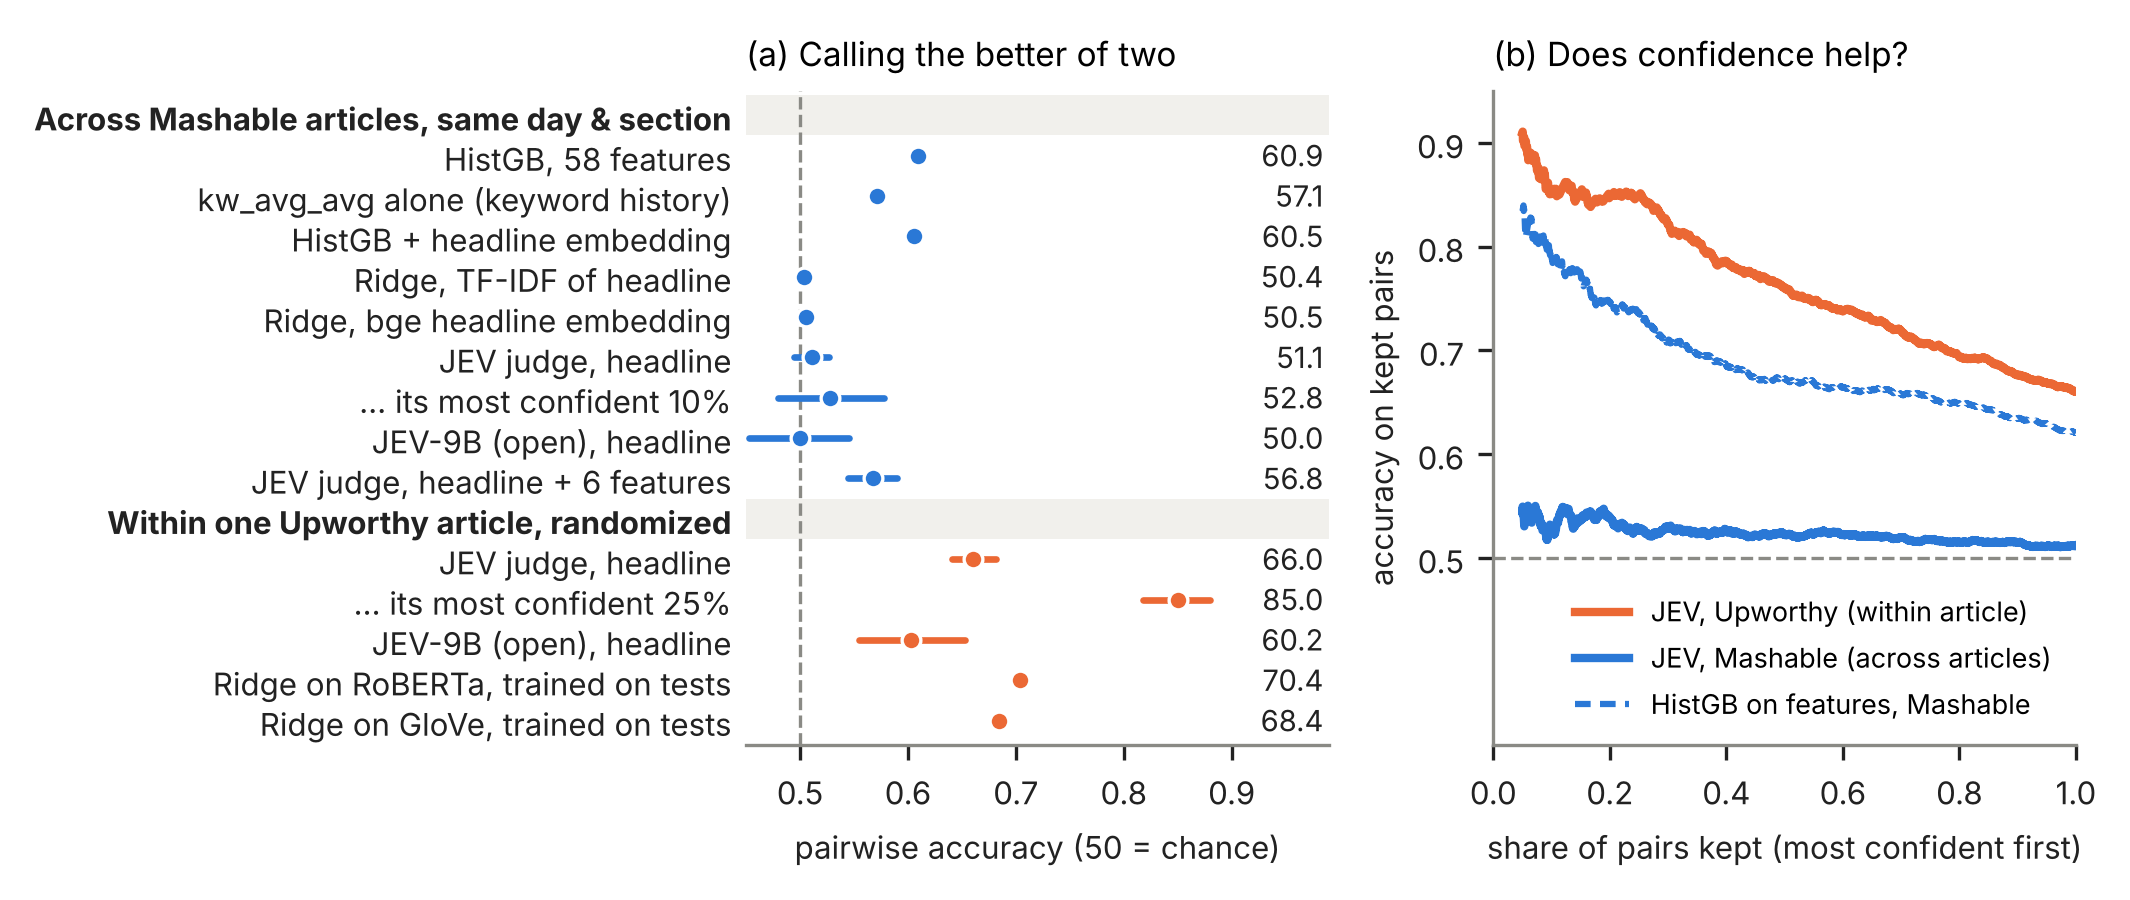
\includegraphics[width=\textwidth]{v19_fig_judge.png}
\caption{RQ3. (a) Pairwise accuracy of scorers on Mashable pairs from the same day and section (past-only
scorers: all such pairs in 2013-07 to 2014-12; judges: 4{,}000 random pairs; with features: 2{,}000) and on
significantly different headline pairs within one randomized Upworthy test (judge: 2{,}000 pairs; ridge: all
pairs, five-fold over articles); 95\% intervals over days or pairs. (b) Accuracy on the pairs a scorer is most
confident about, by the share of pairs kept (judge: larger option probability; HistGB: absolute score
difference).}
\label{fig:judge}
\end{figure*}

\paragraph{From June 2013 on, the headline adds nothing detectable across articles.} In the scored months real
headlines carry no information about which of two articles will be shared more (Fig.~\ref{fig:judge}a,
Table~\ref{tab:six}). Past-only ridge regressions on TF-IDF or bge embeddings of the headline reach an AUC of
0.510 [0.504, 0.516] and 0.510 [0.503, 0.516] and day rankings of 0.008 and 0.014 [0.001, 0.026]. Adding the
embedding to HistGB makes it slightly \emph{worse} (AUC $-$0.0045 [$-$0.0062, $-$0.0028]). The zero-shot judge does
no better: on the 3{,}135 of its 4{,}000 same-day same-section pairs published from 7 June 2013 it is right 48.9\%
[47.3, 50.6] of the time (all 4{,}000: 51.1\%; 4{,}000 same-day pairs: 52.1\%), although its answers are
consistent across option orders (84\%). Its confidence does not help (Fig.~\ref{fig:judge}b): on the tenth of all
4{,}000 pairs it is most confident about it reaches 52.8\%, whereas HistGB is right on 79\% of its own. Given the whole day's lineup, its
probability of ``shared the most'' correlates with log shares at $-$0.003 [$-$0.016, 0.010] within days, and its top
pick lands in the day's top tenth on 11.6\% [9.0, 14.4] of 569 days (random: 11.2\%; HistGB: 35.6\%). On the pairs
that HistGB scores, HistGB is right 62.0\% of the time and the judge 49.1\%; combining the two gives 62.4\%. Given
the headline plus six of the dataset's features, the judge reaches 56.8\% [54.5, 59.0], the same as
\texttt{kw\_avg\_avg} alone on those pairs (55.9\%). A second question wording agrees with the first on 87.5\% of
1{,}000 pairs, and the open-weights JEV-9B is right on 50.0\% [45.2, 54.5] of 400 pairs from the scored months
(API: 48.3\%).

\begin{table}[t]
\centering\footnotesize
\caption{RQ3: six ways headline text could have helped to call popularity across articles, all after the break
(pairs: same day and section; chance 50\%).}
\label{tab:six}
\setlength{\tabcolsep}{2.5pt}
\begin{tabular}{@{}p{0.47\columnwidth}p{0.49\columnwidth}@{}}
\toprule
Test & Result \\
\midrule
Zero-shot judge, pairs & 48.9\% [47.3, 50.6] \\
Zero-shot judge, day lineup & top pick in top tenth 11.6\% (random 11.2\%) \\
Supervised, headline only & 50.4\% (TF-IDF), 50.5\% (bge) \\
Headline added to features & 60.5\% vs.\ 60.9\% without \\
Similar earlier headlines (crowding) & AUC $-$0.0003 [$-$0.0011, 0.0005] \\
New topics (most novel fifth) & headline-only AUC 0.517; with features 0.719 vs.\ 0.722 without \\
\bottomrule
\end{tabular}
\end{table}

\begin{figure}[t]
\centering
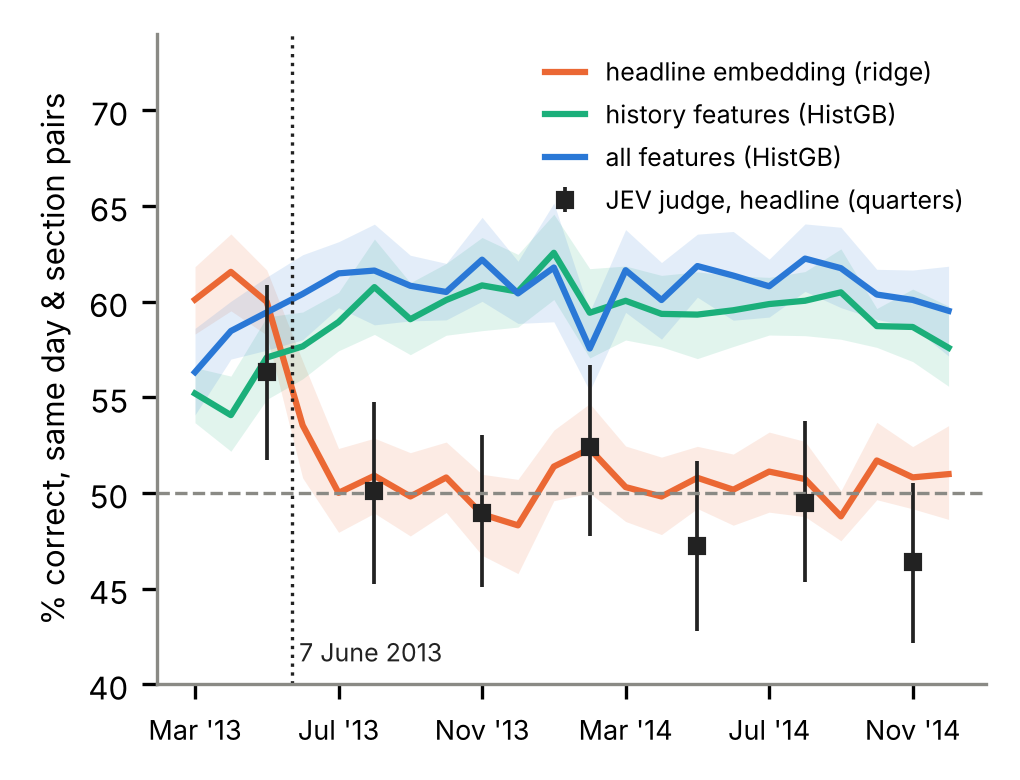
\includegraphics[width=\columnwidth]{v19_fig_regime.png}
\caption{RQ3: accuracy on same-day same-section pairs by publication month, rolling origin from March 2013
(shaded: 95\% intervals over days); squares: zero-shot judge on its judged pairs, by quarter. Headline text is the
best signal until early June 2013 and carries none afterwards.}
\label{fig:regime}
\end{figure}

\paragraph{Until June 2013 it was the best signal: a break in the benchmark.} The judge's accuracy is not uniform
over time (58.5\% and 56.3\% in the first two quarters of 2013, 46--52\% later), which we first took for recall of
older articles. It is not. Starting the rolling origin in March 2013 (Fig.~\ref{fig:regime}), a ridge regression on
headline embeddings that has seen only earlier months orders same-day same-section pairs of March--May 2013
correctly 60.5\% [59.4, 61.7] of the time (TF-IDF: 59.7\%), better than the history features (55.5\%) and than all
58 features (58.1\%; with the embedding added: 61.0\%). In June it drops to 53.5\%, and from July on it is at 49.9\%
(2014: 50.7\%). The change is abrupt. A headline model trained on January--March 2013 correlates with log shares
among a day's articles at 0.31 on average until 6 June 2013 and at 0.02 from 7 June, the least-squares change
point; the dataset's own URL keywords show the same step (0.17 to 0.04), so it is not an artefact of the headlines
we added. The relation did not merely change: the January--March model is right 60.2\% of the time on April--May
and 50.2\% and 50.0\% on later periods, and models trained on later periods reach 50.0--50.4\% on April--May 2013 and
50.1--50.2\% on later ones. The feature models show no break; the history features only improve as history
accumulates. The zero-shot judge follows the headline models: 59.3\% [56.0, 62.9] on pairs before 7 June and 48.9\%
after; on day lineups a within-day correlation of 0.14 [0.12, 0.17] and a top pick in the top tenth on 19\% of days
before, and none after. Its early signal is not verbatim recall: with every headline reworded it is right on 62.0\%
[56.0, 67.6] of 250 early pairs (original wording: 60.8\%; same decision on 87\%), and supervised models that have
seen nothing but January--March show the same pattern. (Asked how often a single article was shared, the judge's
answer correlates with true shares at 0.24 for articles from the first half of 2013 and 0.00 for 2014.) We cannot
explain the break: no dataset feature changes its relation to shares at that date, and a step within days is more
typical of a change in the platform, in distribution on social networks or in how shares were counted than of
readers' tastes drifting. Whatever its cause, it matters for anyone using this benchmark: random cross-validation
blends the two regimes (headline-only AUC 0.53--0.54 instead of 0.51 from July 2013), and a text signal that was
the best single predictor disappeared within a week.

\paragraph{Within an article the headline matters, and the judge sees it.} Asked the same kind of question about
two headlines of one Upworthy article whose click-through differed significantly in a randomized test, the same
judge is right 66.0\% [64.1, 68.2] of the time, and 85.0\% [81.8, 88.0] on its most confident quarter: its
confidence supports selective prediction \citep{geifman2017}, with accuracy rising steadily as coverage falls
(Fig.~\ref{fig:judge}b). It is not
only recalling famous headlines: on pairs in which neither headline won its test it is right 63.4\% (with a winner:
66.8\%). Supervised ridge regressions trained on randomized contrasts reach 70.4\% (RoBERTa) and 68.4\% (GloVe);
adding the judge's verdict to RoBERTa adds about 2 points. A second wording (``Which headline would make more readers
click?'') gives 66.1\% on 1{,}000 of the pairs (first wording on the same pairs: 64.1\%; agreement 84\%). The open-weights JEV-9B is right on 60.3\% [55.5, 65.3] of 400 of the pairs (API on the same
pairs: 63.3\%; agreement 68\%).

\paragraph{Why the two differ.} On 4{,}000 random headline pairs of Upworthy cells, the true log-odds contrast
(observed contrast with its sampling variance removed) has a standard deviation of $\sigma_h=0.42$, and the judge's
verdict (log-odds) correlates $\rho=0.30$ with it. Between two Mashable articles
of one day and section, log shares differ with standard deviation $\sigma_\Delta=1.27$. If headlines moved Mashable
shares as much as Upworthy clicks ($c=1$), they would account for $(0.42/1.27)^2\approx11\%$ of that difference;
a \emph{perfect} headline judge would then be right $\tfrac12+\arcsin(0.33)/\pi=60.6\%$ of the time and this judge
53.1\% [52.7, 53.5]. After the break the judge is right 48.9\% [47.3, 50.6] of the time, which under this model
implies $c$ below about 0.2: wording effects on Mashable shares at most a fifth of those on Upworthy clicks, or a
sense of a good headline that does not carry over. Before the break its 59.3\% exceeds what wording effects of
Upworthy's size could give even at $c=1$, so there the headline must have worked as a description of the
article, its topic and type, rather than as wording. The argument assumes Gaussian effects and is a decomposition, not
a measurement; what it shows is that a judge that clearly sees headline quality need not be able to call popularity
across articles, where wording is a small part of a large difference, and that the pre-break signal was about what
articles were about.

\subsection{Choosing the headline: what an archive is worth (RQ4)}
\label{sec:rq4}
On Upworthy, where headlines were randomized, an idealized archive of 18{,}200 observational headlines (week-demeaned
click-through) reaches a decision accuracy of 66.7\%; a learner trained on randomized contrasts needs 1{,}000 [670,
1{,}810] tests to match it, and with all $\approx$9{,}600 usable tests reaches 68.4\%. An archive of the published
(winning) headlines, as kept by a newsroom that already runs tests, is worth 730 [490, 1{,}130] tests; trained on raw
click-through, the two archives are worth only 520 and 290. The worth grows far more slowly than the archive
(1{,}000 to 18{,}200 headlines: 320 to 1{,}000 tests); a saturating curve fits best and puts a ceiling at about
1{,}200 tests (750--2{,}430), but slow logarithmic growth cannot be ruled out. Used as a prior that experiments
correct \citep{kallus2018}, the archive adds 9 points of accuracy at 25 tests and never costs more than 0.4 points,
whereas pooling the two falls behind the experiments alone from 3{,}200 tests on. Choosing which tests to run by the
archive's predictions or uncertainty does not beat random tests once the archive is the prior.

% ------------------------------------------------------------------
\section{Discussion}
\label{sec:discussion}
\paragraph{What can be called.} Before publication an editor can call a good deal: the model's top pick of the day
is three times as likely as a random pick to be among the day's most shared articles. That skill is about the
article, not its context, and comes mostly from the platform's own history of what similar keywords did. What
cannot be called is the larger part. About three quarters of the variance of log shares is not explained by the
model, the day and the story. That remainder includes unmeasured promotion and seeding as well as the social
influence and chance documented in cultural markets \citep{salganik2006,martin2016}.

\paragraph{Two decisions, two tools.} ``Which articles should we push?'' and ``Which headline should this article
get?'' differ in scale. Across articles, differences in shares are large and come with what the article is and how
its kind has done before; the wording of a headline is a small multiplier on top, and after June 2013 the headline
tells nothing at all. Within an article everything but the wording is fixed, and there a calibrated judge is
informative and knows when it is right. This suggests a division of labour before publication: rank the day's
articles with a model on platform history (top pick 2.1 times the shares of a random article); then choose the
headline with a judge, accept its confident verdicts (85\% right on a quarter of the pairs) and test the rest
\citep{li2026jev}, with an archive of past headlines worth hundreds of tests (RQ4). The second step rests on
Upworthy clicks, not Mashable shares, so for Mashable it is a hypothesis. Reports of headline effects from
randomized tests \citep{matias2021,gligoric2023,banerjee2025} do not imply that headlines help predict popularity,
and a null across articles does not imply that headlines do not matter.

\paragraph{Signals that vanish.} For five months headline text was the best predictor in this benchmark; within a
week it was worth nothing, while the history features kept working. A past-only evaluation shows this; a random
split averages it away. Text-based popularity models need monitoring by period, and results on this benchmark that
involve text should say which period they cover.

\paragraph{Limitations.} Shares were recorded once, in January 2015, so article age and date are confounded, and
the history features use the collection-date shares of earlier articles, which makes their value somewhat
optimistic. Mashable headlines were matched from a sitemap that lists the current headline, which may differ from
the one at publication for some articles. The judge may have seen Mashable articles during training; rewording and
the agreement with models trained only on early 2013 argue against recall as the source of its early signal, but
cannot exclude knowledge of which stories were big. We date the break but cannot explain it, and have no second
source of share counts to check whether measurement changed. We test one judge family (API and open 9B); two question wordings and four prompt formats (headline,
keywords, headline with features, whole day) lead to the same conclusion. Upworthy and Mashable differ in outcome (clicks vs.\ shares), audience and era, which
is why the variance argument leaves $c$ free. The rewordings were written by a language model, not by humans. The same-story pairs are recovered automatically and are about 71\%
precise, judged by two language models, not by humans.

\section{Conclusion}
What can be called before publication on Mashable is real but limited: strictly from the past, a model orders
the day's articles with a correlation of 0.40, and its daily top pick is three times as likely as a random pick to be a
top-tenth article. The skill is article-level and rests mostly on platform history. The real headline, now added to
the benchmark, was the best single signal until 6 June 2013 and adds nothing detectable afterwards, for supervised
text models and for a zero-shot judge alike; the judge's early signal survives rewording and is not recall. On
randomized tests the same judge picks the better headline of one article 66\% of the time, 85\% when most confident.
Choosing which articles to push and choosing a headline are different decisions: the first is served by platform
history, the second by a calibrated judge backed by experiments. And a benchmark can change under a model
overnight: only evaluation that respects time shows it.

\setlength{\bibsep}{0pt}\renewcommand{\bibfont}{\scriptsize}
\bibliographystyle{plainnat}
\bibliography{references}
\end{document}
